\chapter{Cơ chế Higgs: Cách một boson chuẩn thu được khối lượng}

Bây giờ ta kết hợp hai ý tưởng đã được phát triển trong bài giảng trước. Một trường vô hướng phức với đối xứng toàn cục \(U(1)\) bị phá vỡ chứa một dao động hướng tâm có khối lượng và một dao động góc không khối lượng. Một lý thuyết \(U(1)\) bất biến cục bộ chứa một trường chuẩn không khối lượng. Khi trường vô hướng mang điện tích và độ lớn cân bằng của nó khác không, không thể đơn giản cộng gộp các phát biểu này với nhau. Mode góc và trường chuẩn kết hợp với nhau: trường chuẩn trở nên có khối lượng, boson Goldstone biểu kiến không còn là một hạt độc lập nữa, còn mode Higgs hướng tâm vẫn còn lại.

Photon sẽ là boson chuẩn mô hình của ta, nhưng không phải kết luận vật lý của ta. \(U(1)\) điện từ không bị phá vỡ trong chân không, nên photon thực là không khối lượng. Cùng cơ chế ấy tác dụng lên \(W^\pm\) và \(Z\) trong lý thuyết điện yếu, nơi nhóm chuẩn và đa bội vô hướng phức tạp hơn. Mô hình abel làm lộ rõ cơ chế mà không che khuất nó dưới lớp lý thuyết nhóm.

\begin{classroomqa}
\audiencequestion{Liệu phần thảo luận trước có hàm ý rằng cơ chế Higgs cấp khối lượng cho photon thực không?\lecturetimestamp{00:00:23}}
\lecturerresponse{Không. Ta đang hỏi điều gì sẽ xảy ra \emph{nếu} \(U(1)\) gắn với photon ở trong một pha bị phá vỡ. Photon giả định đó sẽ trở nên có khối lượng. Chân không điện từ thực không ở trong pha ấy; thay vào đó, ứng dụng vào vật lý hạt là khối lượng của \(W\) và \(Z\).}
\end{classroomqa}

Đối xứng gắn với bảo toàn điện tích là phép quay pha
\begin{equation}
  \phi(x)\longmapsto e^{i\theta}\phi(x),
\end{equation}
một phép quay nội được gọi là \(U(1)\). Chất siêu dẫn cung cấp một tương tự thực của pha bị phá vỡ. Bên trong nó, trường điện từ có độ sâu xuyên thấu hữu hạn và xét trên những phương diện quan trọng thì ứng xử như một trường có khối lượng. Bên ngoài nó, photon thông thường không khối lượng lại xuất hiện.

\section{Khối lượng có nghĩa gì đối với một trường}

\subsection{Tán sắc và khe hở ở động lượng bằng không}

Trước khi đưa vào trường Higgs, ta nên xác định chính xác điều ta muốn nói bởi khối lượng. Đối với một sóng,
\begin{equation}
  E=\hbar\omega,
  \qquad
  p=\hbar k,
  \label{eq:l08-quantum-wave}
\end{equation}
vì vậy đồ thị \((E,p)\) và đồ thị \((\omega,k)\) chứa cùng một thông tin, sai khác chỉ ở các hệ số \(\hbar\). Trong không gian trống, một kích thích tương đối tính không khối lượng tuân theo
\begin{equation}
  E=c|p|,
  \qquad
  \omega=c|k|.
  \label{eq:l08-massless-dispersion}
\end{equation}
Hai dấu của \(k\) phân biệt hai hướng lan truyền đối ngược. Điểm cốt yếu là \(\omega\) tiến về 0 cùng với \(k\).

Một hạt tương đối tính có khối lượng tuân theo
\begin{equation}
  E^2=c^2p^2+m^2c^4.
  \label{eq:l08-massive-dispersion}
\end{equation}
Trong các đơn vị \(c=\hbar=1\),
\begin{equation}
  \omega^2=k^2+m^2.
\end{equation}
Tại \(k=0\), năng lượng là \(E=mc^2\), hay đơn giản là \(m\) trong đơn vị tự nhiên. Vì thế, khối lượng là khe hở năng lượng khác không của mode có động lượng bằng không.

\begin{figure}[htbp]
\centering
\begin{adjustbox}{max width=\linewidth}
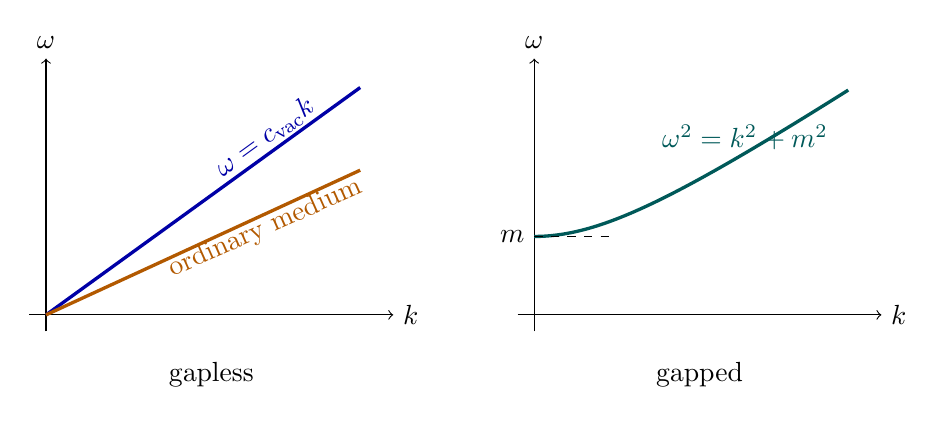
\begin{tikzpicture}[x=1.05cm,y=1.05cm]
  \begin{scope}
    \draw[->] (-0.2,0) -- (4.2,0) node[right] {\(k\)};
    \draw[->] (0,-0.2) -- (0,3.1) node[above] {\(\omega\)};
    \draw[very thick,blue!65!black] (0,0) -- (3.8,2.75);
    \draw[very thick,orange!70!black] (0,0) -- (3.8,1.75);
    \node[blue!65!black,rotate=36] at (2.65,2.15)
      {\(\omega=c_{\rm vac}k\)};
    \node[orange!70!black,rotate=24] at (2.65,1.05)
      {ordinary medium};
    \node[below] at (2,-0.45) {gapless};
  \end{scope}
  \begin{scope}[xshift=6.2cm]
    \draw[->] (-0.2,0) -- (4.2,0) node[right] {\(k\)};
    \draw[->] (0,-0.2) -- (0,3.1) node[above] {\(\omega\)};
    \draw[very thick,domain=0:3.8,samples=120,smooth,teal!70!black]
      plot (\x,{sqrt(0.9+0.45*\x*\x)});
    \draw[dashed] (0,0.95) -- (1.0,0.95);
    \node[left] at (0,0.95) {\(m\)};
    \node[teal!70!black] at (2.55,2.15)
      {\(\omega^2=k^2+m^2\)};
    \node[below] at (2,-0.45) {gapped};
  \end{scope}
\end{tikzpicture}
\end{adjustbox}
\caption{Thay đổi tốc độ lan truyền sẽ làm thay đổi độ dốc của một quan hệ tán sắc không có khe hở. Gán khối lượng cho kích thích sẽ mở ra một khe hở khác không tại \(k=0\).}
\label{fig:l08-dispersion}
\end{figure}

Một vật liệu trong suốt thông thường có thể làm giảm vận tốc pha của sóng mà không tạo ra khe hở khối lượng tương đối tính này. Tại một biên, tần số tới được giữ cố định, còn số sóng thì tự điều chỉnh theo quan hệ tán sắc của môi trường. Thay đổi độ dốc không đồng nghĩa với việc nâng tung độ gốc lên.
\editorialnote{Một vật liệu có thể có vài nhánh điện từ, và plasma hoặc môi trường cộng hưởng có thể có một khe hở tần số plasma khác không. Phép so sánh trong bài giảng cụ thể là giữa một nhánh khúc xạ thông thường và đáp ứng siêu dẫn. Tổng quát hơn, tính không khe hở có nghĩa là \(\omega(k)\to0\) khi \(k\to0\); không phải trong mọi môi trường phi tương đối tính đều cần tính tuyến tính chính xác.}

\begin{classroomqa}
\audiencequestion{Có phải photon thu được khối lượng mỗi khi nó truyền qua vật chất, chẳng hạn qua một lăng kính không?\lecturetimestamp{00:03:02}}
\lecturerresponse{Không. Hiện tượng khúc xạ có thể làm thay đổi quan hệ giữa tần số và số sóng, và do đó thay đổi tốc độ lan truyền, trong khi nhánh đó vẫn đi qua \(\omega=0\) tại \(k=0\). Trái lại, một pha siêu dẫn làm cho đáp ứng điện từ có một nghịch đảo độ sâu xuyên thấu hữu hạn, là tương tự của khối lượng.}
\end{classroomqa}

\begin{classroomqa}
\audiencequestion{Đối với ánh sáng có tần số cố định đi vào thủy tinh, có phải số sóng là đại lượng thay đổi không?\lecturetimestamp{00:09:20}}
\lecturerresponse{Đúng. Tính bất biến theo tịnh tiến thời gian tại một mặt phân cách đứng yên giữ cho tần số không đổi. Vì đường cong tán sắc có độ dốc khác trong thủy tinh, cùng một \(\omega\) tương ứng với một \(k\) khác, và do đó với một bước sóng khác.}
\end{classroomqa}

Độ dốc
\begin{equation}
  v_g=\frac{d\omega}{dk}
\end{equation}
là vận tốc nhóm của một gói sóng. Nếu độ dốc ấy biến thiên theo \(k\), các thành phần Fourier khác nhau sẽ chuyển động với những tốc độ khác nhau và gói sóng sẽ tán ra. Đó là lý do quan hệ \(\omega(k)\) được gọi là \emph{quan hệ tán sắc}.

\begin{classroomqa}
\audiencequestion{Đường cong ấy được gọi là gì, và độ dốc của nó biểu diễn điều gì?\lecturetimestamp{00:11:02}}
\lecturerresponse{Đường cong đó là quan hệ tán sắc. Đạo hàm của nó \(d\omega/dk\) là vận tốc nhóm. Một độ dốc không đổi cho cùng một vận tốc đối với mọi bước sóng; một độ dốc biến thiên làm gói sóng loe ra. Với mục đích hiện tại, điểm phân biệt có tính quyết định là liệu đường cong có chạm tới gốc tọa độ hay có một khe hở.}
\end{classroomqa}

\subsection{Một dao động đồng nhất là một hạt đứng yên}

Mode \(k=0\) có bước sóng vô hạn: trường bị dịch đi cùng một lượng ở mọi nơi. Hãy thả tự do một dịch chuyển đồng nhất. Nếu trường dao động với tần số khác không, lượng tử tương ứng có năng lượng nghỉ khác không và là có khối lượng. Nếu không có lực phục hồi theo hướng đó, tần số triệt tiêu và mode là không khối lượng.

Phát biểu này là cổ điển. Nó không đòi hỏi các hạt tách biệt trong không gian phải ở trong một chồng chập lượng tử. Một cấu hình trường cổ điển đồng nhất đơn giản chỉ là một giá trị trường được lặp lại khắp không gian.

\begin{classroomqa}
\audiencequestion{Nếu toàn bộ một trường cùng bị dịch chuyển, điều đó có giống với sự vướng víu lượng tử không?\lecturetimestamp{00:10:04}}
\lecturerresponse{Không. Một trường cổ điển đồng nhất là một cấu hình cổ điển duy nhất. Sự vướng víu tương quan các khả năng lượng tử phân biệt, chẳng hạn các cấu hình spin lên--xuống và xuống--lên. Việc chuẩn bị cùng một giá trị trường tại nhiều điểm tự nó không phải là vướng víu, cũng không hàm ý một đáp ứng nhân quả tức thời.}
\end{classroomqa}

Đối với một trường thực được chuẩn hoá chuẩn tắc,
\begin{equation}
  \mathcal L
  =\frac12\partial_\mu\varphi\,\partial^\mu\varphi-V(\varphi),
\end{equation}
khai triển quanh một trạng thái cân bằng \(\varphi_0\):
\begin{equation}
  V(\varphi_0+\eta)
  =V(\varphi_0)
   +\frac12V''(\varphi_0)\eta^2+\cdots.
\end{equation}
Số hạng tuyến tính triệt tiêu tại điểm cực tiểu, và phương trình trường cho
\begin{equation}
  \omega^2=\bm{k}^2+m^2,
  \qquad
  m^2=V''(\varphi_0).
  \label{eq:l08-curvature-mass}
\end{equation}
Vì thế, khối lượng là độ cong của thế năng theo hướng chuyển động. Một hướng phẳng có độ cong bằng không và cho ra một mode không khối lượng.

\section{Trường vô hướng phức bị phá vỡ}

\subsection{Chuyển động theo phương bán kính và chuyển động góc}

Hãy viết một trường vô hướng phức trong tọa độ Descartes và tọa độ cực:
\begin{equation}
  \phi=\phi_R+i\phi_I=\rho e^{i\alpha},
  \qquad
  \phi^*=\phi_R-i\phi_I=\rho e^{-i\alpha}.
  \label{eq:l08-polar-field}
\end{equation}
Mặt phẳng phức là một không gian trường \emph{nội}. Tại mỗi điểm không-thời gian vật lý \(x\), cặp
\((\phi_R(x),\phi_I(x))\)
chỉ định một điểm trong mặt phẳng nội đó. Không trục nội nào là một phương trong phòng thí nghiệm.

\begin{figure}[htbp]
\centering
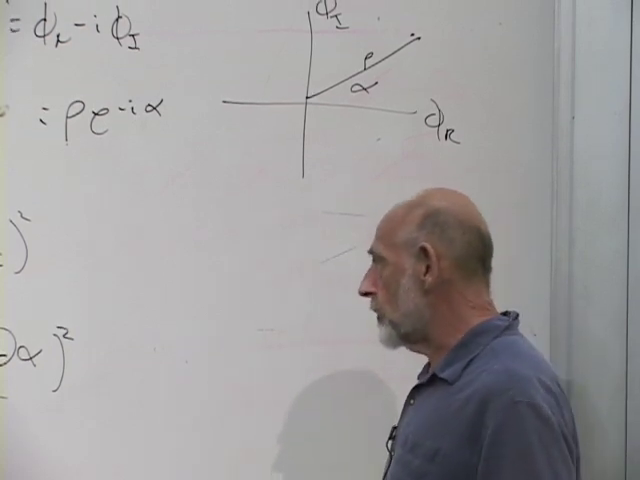
\includegraphics[width=0.72\textwidth]{lecture_08_figure_02.png}
\caption{Trường vô hướng phức được biểu diễn trong mặt phẳng \((\phi_R,\phi_I)\) nội của nó. Bán kính là \(\rho\), còn \(\alpha\) là pha nội.}
\lectureframe{00:24:41}
\label{fig:l08-internal-plane}
\end{figure}

Số hạng động học của trường vô hướng trở thành
\begin{align}
  \partial_\mu\phi^*\,\partial^\mu\phi
  &=
  \partial_\mu\phi_R\,\partial^\mu\phi_R
  +\partial_\mu\phi_I\,\partial^\mu\phi_I
  \notag\\
  &=
  \partial_\mu\rho\,\partial^\mu\rho
  +\rho^2\partial_\mu\alpha\,\partial^\mu\alpha.
  \label{eq:l08-polar-kinetic}
\end{align}
Một thế năng bất biến \(U(1)\) toàn cục phụ thuộc vào
\(\phi^*\phi=\rho^2\), chứ không phụ thuộc vào \(\alpha\). Chẳng hạn,
\begin{equation}
  V(\phi)
  =\lambda\left(\phi^*\phi-\frac{f^2}{2}\right)^2,
  \qquad \lambda>0.
  \label{eq:l08-mexican-hat}
\end{equation}
Các cực tiểu của nó tạo thành một vòng tròn. Quy luật này bất biến dưới một phép quay pha chung, nhưng việc chọn một pha cân bằng sẽ chọn ra một điểm trên vòng tròn.

\begin{figure}[htbp]
\centering
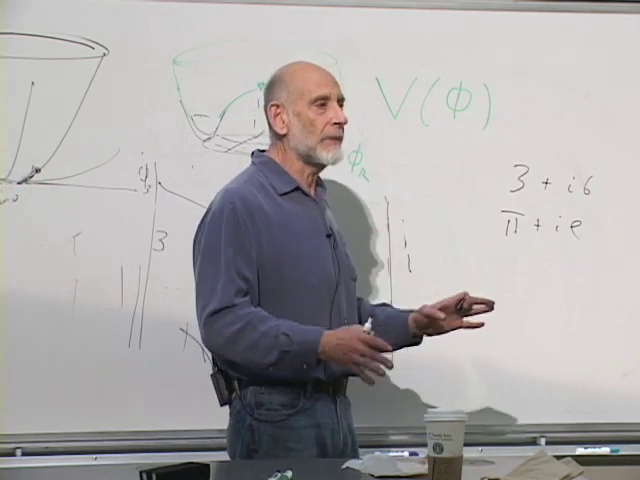
\includegraphics[width=0.78\textwidth]{lecture_08_figure_03.png}
\caption{Các phác họa thế năng hướng tâm trên bảng. Thế năng đối xứng dưới các phép quay của giá trị trường nội, mặc dù bản thân trường không nhất thiết phải nằm tại gốc tọa độ.}
\lectureframe{00:34:22}
\label{fig:l08-radial-potential-board}
\end{figure}

\begin{figure}[htbp]
\centering
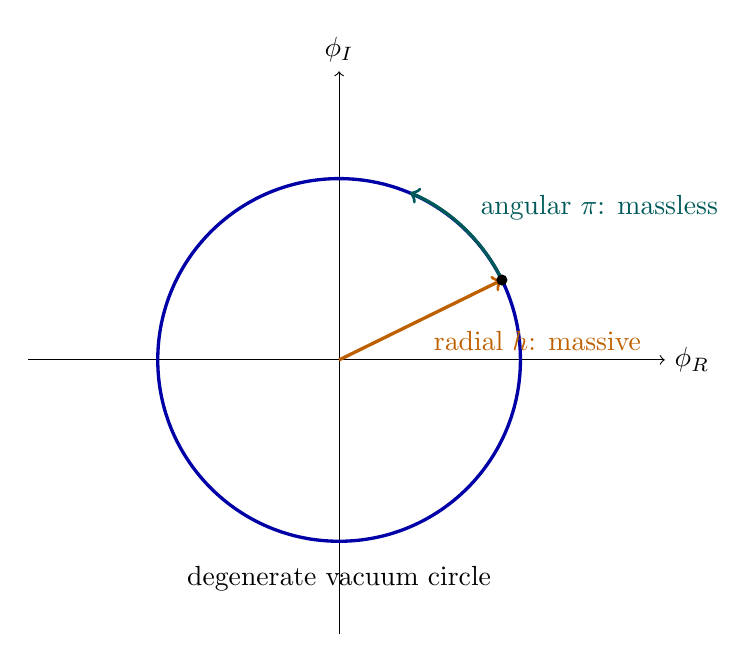
\begin{tikzpicture}[x=0.94cm,y=0.94cm]
  \draw[->] (-4.2,0) -- (4.4,0) node[right] {\(\phi_R\)};
  \draw[->] (0,-3.7) -- (0,3.9) node[above] {\(\phi_I\)};
  \draw[very thick,blue!65!black] (0,0) circle (2.45);
  \draw[->,very thick,orange!75!black] (0,0) -- (2.2,1.08);
  \draw[->,very thick,teal!70!black]
    (2.2,1.08) arc[start angle=26,end angle=67,radius=2.45];
  \node[orange!75!black,below right] at (1.15,0.52)
    {radial \(h\): massive};
  \node[teal!70!black,above right] at (1.78,1.76)
    {angular \(\pi\): massless};
  \fill (2.2,1.08) circle (2pt);
  \node[below] at (0,-2.65) {degenerate vacuum circle};
\end{tikzpicture}
\caption{Lý thuyết bị phá vỡ toàn cục có độ cong theo pháp tuyến với vòng tròn chân không nhưng không có độ cong dọc theo nó. Mode Higgs hướng tâm là có khối lượng; mode Goldstone góc là không khối lượng.}
\label{fig:l08-radial-angular}
\end{figure}

Đặt
\begin{equation}
  \phi(x)=\frac{f+h(x)}{\sqrt2}
           e^{i\pi(x)/f}.
  \label{eq:l08-canonical-polar}
\end{equation}
Gần chân không đã chọn, \(h\) đo độ dịch chuyển hướng tâm còn \(\pi\) đo độ dịch chuyển tiếp tuyến với các thứ nguyên chuẩn tắc. Thế vào Eq.~\eqref{eq:l08-polar-kinetic} ta được
\begin{equation}
  \partial_\mu\phi^*\,\partial^\mu\phi
  =
  \frac12(\partial_\mu h)^2
  +\frac12\left(1+\frac{h}{f}\right)^2
            (\partial_\mu\pi)^2.
  \label{eq:l08-global-expanded}
\end{equation}
Thế năng trong Eq.~\eqref{eq:l08-mexican-hat} cho
\begin{equation}
  m_h^2=2\lambda f^2,
  \qquad
  m_\pi^2=0.
  \label{eq:l08-global-masses}
\end{equation}
Ở các năng lượng thấp hơn rất xa \(m_h\), chuyển động hướng tâm tốn năng lượng, nên tạm thời ta có thể cố định \(h=0\). Lagrangian còn lại chỉ chứa \(\frac12(\partial\pi)^2\), không có hạng \(\pi^2\). Đây là boson Goldstone.\editorialnote{Ở hai chỗ, phần giải thích bằng lời đã đảo ngược tên gọi và nói rằng việc nuốt Goldstone làm cho boson Higgs có khối lượng. Phép tính trên bảng và phần còn lại của bài giảng xác lập kết quả được chủ ý: độ cong hướng tâm đã làm cho mode Higgs có khối lượng, còn boson chuẩn tiếp nhận mode Goldstone và trở nên có khối lượng.}

\begin{classroomqa}
\audiencequestion{Đây có phải là sự phá vỡ đối xứng tự phát duy nhất trong Mô hình Chuẩn không?\lecturetimestamp{00:16:39}}
\lecturerresponse{Pha Higgs điện yếu là cơ chế phá vỡ đối xứng đã được xác lập liên quan ở đây. Đối xứng thực sự của nó là \(SU(2)_L\times U(1)_Y\), chứ không phải \(U(1)\) đơn lẻ này, và QCD còn có cấu trúc chân không bổ sung như sự phá vỡ đối xứng chiral. Ví dụ abel là một mô hình được rút gọn có chủ ý của cơ chế boson chuẩn.}
\end{classroomqa}

\begin{classroomqa}
\audiencequestion{Higgs có cấp khối lượng cho mọi hạt, kể cả chính nó, không?\lecturetimestamp{00:17:11}}
\lecturerresponse{Câu trả lời cần phân biệt theo nghĩa vừa có vừa không. Đối xứng điện yếu cấm các khối lượng trần cho \(W\), \(Z\) và các fermion của Mô hình Chuẩn; khối lượng của chúng xuất hiện sau khi trường Higgs nhận một độ lớn cân bằng khác không. Khối lượng Higgs hướng tâm đến từ độ cong của chính thế năng của nó. Các hạt giả thuyết khác có thể mang những khối lượng được đối xứng cho phép không liên quan đến cơ chế này.}
\end{classroomqa}

Bài giảng gắn những khối lượng được đối xứng cho phép như vậy với các hạt có thể rất nặng và khó quan sát, đồng thời nêu vật chất tối như một ví dụ có thể có. Đó là một động cơ, không phải một dự đoán khối lượng.
\editorialnote{Thang khối lượng của vật chất tối vẫn chưa biết. Gợi ý trong bài giảng về một hạt cỡ một nghìn lần khối lượng proton là suy đoán mang tính lịch sử, không phải một tính chất của vật chất tối đã được xác lập bằng thực nghiệm.}

\begin{classroomqa}
\audiencequestion{\(\rho\) có phải là một bán kính vật lý không, hay nó là giá trị trường? Chính xác thì cái gì đối xứng hướng tâm?\lecturetimestamp{00:33:08}}
\lecturerresponse{Tại mỗi điểm không-thời gian, giá trị trường là một điểm trong một mặt phẳng phức phụ trợ, và \(\rho=|\phi|\) là khoảng cách từ điểm đó đến gốc tọa độ. \emph{Thế năng} là đối xứng hướng tâm trong mặt phẳng nội này: mọi điểm có cùng \(\rho\) đều có cùng thế năng. Bán kính này không phải là một khoảng cách trong không gian thông thường.}
\end{classroomqa}

\begin{classroomqa}
\audiencequestion{Liệu một cú kích hướng tâm đủ mạnh có thể đưa trường vượt qua cực đại ở tâm sang phía bên kia của thế năng không?
\lecturetimestamp{00:36:00}}
\lecturerresponse{Về nguyên tắc, một cấu hình cục bộ có đủ năng lượng có thể vượt qua rào thế. Để đưa một trường vĩ mô đồng nhất vượt qua nó sẽ cần một năng lượng khổng lồ, và một nhiễu động mạnh điển hình sẽ phát tán năng lượng vào nhiều mode trường thay vì tới được điểm đối diện một cách kết hợp. Xấp xỉ năng lượng thấp cố định \(\rho\) chính vì những lệch hướng tâm như vậy không thể tiếp cận được ở đó.}
\end{classroomqa}

\section{Vì sao mặt phẳng phức không phải là không-thời gian}

Sự phân biệt giữa tọa độ vật lý và tọa độ nội đáng để bài giảng dừng lại nhấn mạnh đầy đủ. Một trường vô hướng được gọi là vô hướng vì nó bất biến dưới các phép quay của các trục tọa độ vật lý. Hai trường vô hướng thực \(\phi_R(x)\) và \(\phi_I(x)\) vẫn là hai vô hướng dưới các phép quay đó. Ta có thể gộp chúng thành một số phức, nhưng cách ghi chép này không biến chúng thành các thành phần của một vectơ không gian.

Phép biến đổi \(U(1)\) toàn cục xoay các \emph{giá trị} của trường:
\begin{equation}
\begin{aligned}
  \phi(x)&\longmapsto e^{i\theta}\phi(x),
  \\
  \rho(x)&\longmapsto\rho(x),
  \\
  \alpha(x)&\longmapsto\alpha(x)+\theta.
\end{aligned}
  \label{eq:l08-global-shift}
\end{equation}
Cùng một hằng số \(\theta\) được dùng tại mọi điểm không-thời gian. Do đó,
\(\partial_\mu\alpha\) không đổi. Đây là một đối xứng của cả thế năng
và hạng động năng thông thường. Một khi cho phép \(\theta\) phụ thuộc vào
\(x\), đạo hàm sẽ phát hiện sự biến thiên ấy, và lập luận thay đổi.

\section{Địa phương hóa phép quay pha}

\subsection{Đạo hàm thông thường không còn bất biến}

Hãy đặt
\begin{equation}
  \phi'(x)=e^{i\theta(x)}\phi(x).
  \label{eq:l08-local-phase}
\end{equation}
Khi đó
\begin{equation}
  \partial_\mu\phi'
  =e^{i\theta}
    \left(\partial_\mu\phi+i\,\partial_\mu\theta\,\phi\right).
  \label{eq:l08-ordinary-derivative-fails}
\end{equation}
Hạng phụ tỉ lệ với \(\partial_\mu\theta\) ngăn không cho
\(\partial_\mu\phi\) biến đổi giống như \(\phi\). Vì vậy
\(\partial_\mu\phi^*\partial^\mu\phi\) không bất biến dưới các phép quay
pha cục bộ tùy ý.

\begin{figure}[htbp]
\centering
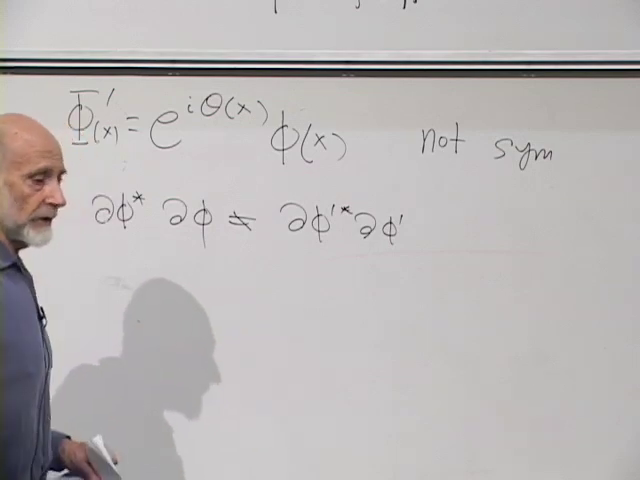
\includegraphics[width=0.78\textwidth]{lecture_08_figure_04.png}
\caption{Bảng ghi lại phép biến đổi pha cục bộ và việc
hạng đạo hàm thông thường không còn bất biến.}
\lectureframe{00:46:49}
\label{fig:l08-local-not-symmetry}
\end{figure}

Đưa vào một thế vectơ và cố định nhất quán một quy ước:
\begin{equation}
  D_\mu=\partial_\mu+i g A_\mu,
  \qquad
  A_\mu'=A_\mu-\frac1g\partial_\mu\theta.
  \label{eq:l08-covariant-convention}
\end{equation}
Khi đó
\begin{align}
  D_\mu'\phi'
  &=
  \left(\partial_\mu+i g A_\mu'\right)
  e^{i\theta}\phi
  \notag\\
  &=
  e^{i\theta}
  \left[
    \partial_\mu\phi+i(\partial_\mu\theta)\phi
    +i g A_\mu\phi-i(\partial_\mu\theta)\phi
  \right]
  \notag\\
  &=e^{i\theta}D_\mu\phi.
  \label{eq:l08-covariant-transform}
\end{align}
Các hạng không mong muốn triệt tiêu nhau. Đạo hàm liên hợp là
\begin{equation}
  (D_\mu\phi)^*
  =(\partial_\mu-i g A_\mu)\phi^*,
\end{equation}
và pha đối dấu của nó triệt tiêu trong tích
\begin{equation}
  (D_\mu\phi)^*D^\mu\phi.
\end{equation}

\begin{classroomqa}
\audiencequestion{Trong bài giảng trước, phép biến đổi của trường chuẩn có phải đã được viết với dấu ngược lại không?\lecturetimestamp{00:48:04}}
\lecturerresponse{Việc đồng thời đảo dấu trong \(D_\mu\) và trong
luật biến đổi chỉ là một quy ước. Với
\(D_\mu=\partial_\mu+i gA_\mu\) và
\(\phi'=e^{i\theta}\phi\), tính nhất quán đòi hỏi
\(A_\mu'=A_\mu-g^{-1}\partial_\mu\theta\). Quy ước thay thế cũng hoạt động
tốt như nhau nếu mọi dấu đều được đổi cùng nhau.}
\end{classroomqa}

\begin{classroomqa}
\audiencequestion{Việc dùng dạng viết hoa hay viết thường của
\(\phi\) trên bảng có đánh dấu một trường khác không?\lecturetimestamp{00:55:02}}
\lecturerresponse{Không có sự phân biệt nào được hàm ý. Hình dạng chữ thay đổi là do
cách viết tay, không phải một phép toán bổ sung hay một vô hướng thứ hai. Những phân biệt
có ý nghĩa là dấu prime, dấu sao liên hợp phức và chỉ số không-thời gian.}
\end{classroomqa}

\begin{classroomqa}
\audiencequestion{Liên hợp phức có phải là cùng một phép toán với việc nâng hoặc
hạ chỉ số Lorentz trong hạng động năng không?
\lecturetimestamp{00:56:50}}
\lecturerresponse{Không. Dấu sao liên hợp trường phức nội tại.
Các chỉ số Lorentz được nâng bằng metric không-thời gian:
\(D^\mu=g^{\mu\nu}D_\nu\). Một vô hướng Lorentz cần phép co
\((D_\mu\phi)^*D^\mu\phi\); cả hai phép toán đều có mặt và phục vụ những
mục đích khác nhau.}
\end{classroomqa}

\subsection{Trường chuẩn có động lực học riêng}

Cường độ trường
\begin{equation}
  F_{\mu\nu}=\partial_\mu A_\nu-\partial_\nu A_\mu
  \label{eq:l08-field-strength}
\end{equation}
là bất biến chuẩn vì hai đạo hàm bậc hai hỗn hợp của \(\theta\)
triệt tiêu nhau. Các thành phần thời gian--không gian của nó chứa điện trường, còn các
thành phần không gian--không gian chứa từ trường. Vì vậy điện động lực học vô hướng có dạng
\begin{equation}
  \mathcal L
  =(D_\mu\phi)^*D^\mu\phi
  -V(\phi^*\phi)
  -\frac14F_{\mu\nu}F^{\mu\nu}.
  \label{eq:l08-abelian-higgs}
\end{equation}
Trường mang điện ở đây là boson. Nó không phải trường electron, vốn là một
fermion. Một hạt nhân heli mang điện hoặc một ngưng tụ cặp Cooper minh họa
cách một bậc tự do boson mang điện có thể xuất hiện.

Trước khi phá vỡ đối xứng, hạng của trường chuẩn chứa các đạo hàm của \(A_\mu\)
nhưng không có hạng khối lượng trực tiếp. Ta có thể thử thêm
\begin{equation}
  \frac12m_A^2A_\mu A^\mu,
\end{equation}
nhưng dưới phép biến đổi trong Eq.~\eqref{eq:l08-covariant-convention},
\begin{equation}
  A_\mu A^\mu
  \longmapsto
  \left(A_\mu-\frac1g\partial_\mu\theta\right)
  \left(A^\mu-\frac1g\partial^\mu\theta\right),
  \label{eq:l08-bare-mass-fails}
\end{equation}
điều này không bằng \(A_\mu A^\mu\). Khối lượng trần của boson chuẩn bị cấm
bởi đối xứng cục bộ.

\begin{figure}[htbp]
\centering
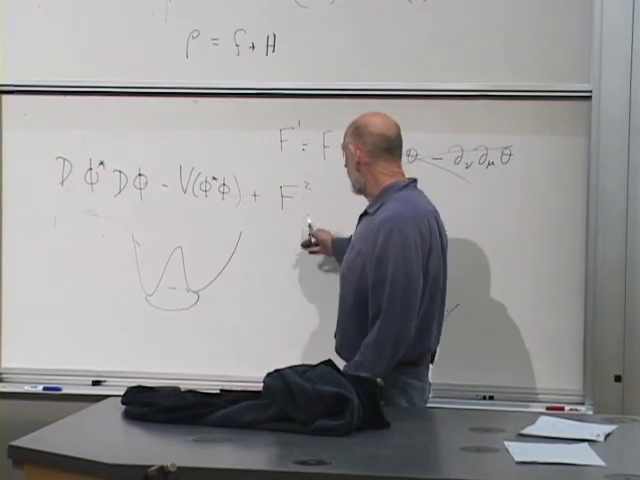
\includegraphics[width=0.76\textwidth]{lecture_08_figure_05.png}
\caption{Một trạng thái bảng đã được kiểm chứng cho thấy sự cản trở này: dưới một phép biến đổi chuẩn,
\(A_\mu A^\mu\) trở thành một bình phương có chứa
\(\partial_\mu\theta\), nên một khối lượng vectơ trần không bất biến.}
\lectureframe{01:07:30}
\label{fig:l08-bare-mass-board}
\end{figure}

\section{Cơ chế Higgs}

\subsection{Đạo hàm hiệp biến sinh ra khối lượng}

Quay lại thế bị phá vỡ và dùng tham số hóa được chuẩn hóa
chính tắc
\begin{equation}
  \phi(x)=\frac{f+h(x)}{\sqrt2}
  e^{i\pi(x)/f}.
\end{equation}
Đạo hàm hiệp biến của nó là
\begin{equation}
  D_\mu\phi
  =
  \frac{e^{i\pi/f}}{\sqrt2}
  \left[
    \partial_\mu h
    +i(f+h)
      \left(\frac{\partial_\mu\pi}{f}+gA_\mu\right)
  \right].
  \label{eq:l08-covariant-polar}
\end{equation}
Do đó,
\begin{equation}
\begin{aligned}
  (D_\mu\phi)^*D^\mu\phi
  ={}&
  \frac12(\partial_\mu h)^2
  \\
  &+\frac12(f+h)^2
    \left(\frac{\partial_\mu\pi}{f}+gA_\mu\right)
  \\
  &\hspace{4.2em}\times
    \left(\frac{\partial^\mu\pi}{f}+gA^\mu\right).
\end{aligned}
  \label{eq:l08-higgs-kinetic}
\end{equation}

Hạng quyết định xuất hiện trước bất kỳ lựa chọn chuẩn nào:
\begin{equation}
  \frac12g^2f^2 A_\mu A^\mu.
  \label{eq:l08-vector-mass-term}
\end{equation}
So sánh nó với dạng Proca
\(\frac12m_A^2A_\mu A^\mu\), ta được
\begin{equation}
  \boxed{m_A=g f}.
  \label{eq:l08-vector-mass}
\end{equation}
Khai triển này cũng sinh ra các tương tác
\(g^2fh A_\mu A^\mu\) và
\(\frac12g^2h^2A_\mu A^\mu\). Vì vậy khối lượng vectơ không phải là một sự
vi phạm đối xứng chuẩn tùy tiện. Nó xuất phát từ một hạng động năng vô hướng
bất biến chuẩn được xét trong một pha có độ lớn cân bằng khác không \(f\).

\begin{figure}[htbp]
\centering
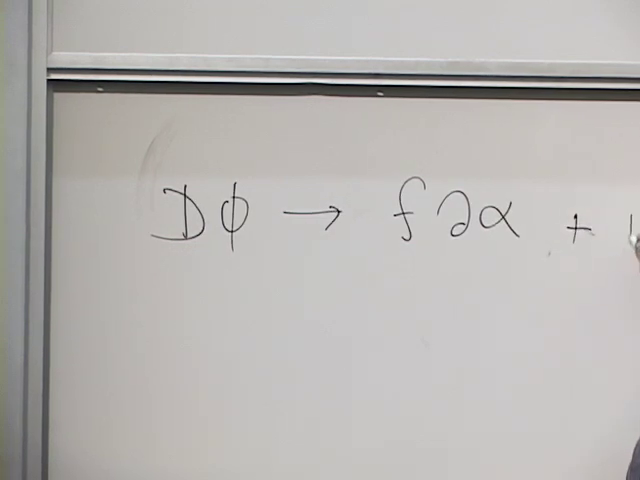
\includegraphics[width=0.78\textwidth]{lecture_08_figure_06.png}
\caption{Trên bảng, phần đóng góp \(f^2A^2\) được tách riêng trong
\((D\phi)^*(D\phi)\). Các hệ số số học phụ thuộc vào cách chuẩn hóa trường vô hướng và
hằng ghép chuẩn; với các Eq.~\eqref{eq:l08-canonical-polar}
và \eqref{eq:l08-covariant-convention}, kết quả là \(m_A=gf\).}
\lectureframe{01:10:10}
\label{fig:l08-generated-mass-board}
\end{figure}

Bài giảng hấp thụ \(g\) và một số hệ số \(\sqrt2\) vào kí hiệu trên bảng
của mình, nên trong lúc xác định khối lượng nó luân phiên trong chốc lát giữa \(f\), \(2f\) và \(\sqrt2f\).
Những hệ số ấy không có ý nghĩa bất biến cho đến khi cách chuẩn hóa
động năng và thế năng được nêu rõ. Kết quả bền vững là
\(m_A\propto gf\); Eq.~\eqref{eq:l08-vector-mass} cho hệ số đối với
quy ước được dùng ở đây.

\subsection{Pha được hấp thụ}

Dưới một phép biến đổi chuẩn, biến pha biến đổi theo
\begin{equation}
  \pi'(x)=\pi(x)+f\,\theta(x).
\end{equation}
Chọn
\begin{equation}
  \theta(x)=-\frac{\pi(x)}{f}.
  \label{eq:l08-unitary-gauge-choice}
\end{equation}
Khi đó \(\pi'=0\). Đây là chuẩn đơn nhất, trong đó
\begin{equation}
  \phi'(x)=\frac{f+h(x)}{\sqrt2}
\end{equation}
là thực, và Eq.~\eqref{eq:l08-higgs-kinetic} rút gọn thành
\begin{equation}
  (D_\mu\phi')^*D^\mu\phi'
  =
  \frac12(\partial_\mu h)^2
  +\frac12g^2(f+h)^2A_\mu'A^{\prime\mu}.
  \label{eq:l08-unitary-gauge-lagrangian}
\end{equation}
Trường Goldstone góc đã biến mất khỏi danh sách các biến độc lập,
trong khi khối lượng vectơ vẫn còn.

Trong bài giảng, điều này trước hết được minh họa trong giới hạn năng lượng thấp
\(\rho=f\), khi đó
\begin{align}
  \phi&=f e^{i\alpha},
  \notag\\
  D_\mu\phi
  &=if e^{i\alpha}
    \left(\partial_\mu\alpha+gA_\mu\right),
  \notag\\
  (D_\mu\phi)^*
  &=-if e^{-i\alpha}
    \left(\partial_\mu\alpha+gA_\mu\right).
  \label{eq:l08-frozen-radius}
\end{align}
Tích của chúng là
\begin{equation}
  f^2
  \left(\partial_\mu\alpha+gA_\mu\right)
  \left(\partial^\mu\alpha+gA^\mu\right).
\end{equation}
Chọn \(\theta=-\alpha\) thì còn lại \(g^2f^2A_\mu'A^{\prime\mu}\).

\begin{figure}[htbp]
\centering
\includegraphics[width=0.82\textwidth]{lecture_08_figure_07.png}
\caption{Trạng thái bảng đầy đủ khi bán kính bị cố định: các đạo hàm hiệp biến
chứa đồng thời đạo hàm pha và thế vectơ. Tiếp theo bài giảng
chọn \(\theta=-\alpha\), loại bỏ pha và để lại hạng khối lượng vectơ.}
\lectureframe{01:16:20}
\label{fig:l08-frozen-radius-board}
\end{figure}

\begin{classroomqa}
\audiencequestion{Có thể viết lại toàn bộ Lagrangian theo các biến làm cho
sự biến mất của mode góc trở nên hiển nhiên không?
\lecturetimestamp{01:13:49}}
\lecturerresponse{Có. Trong các biến cực, pha chỉ xuất hiện thông qua tổ hợp
bất biến chuẩn
\(\partial_\mu\alpha+gA_\mu\). Một phép biến đổi chuẩn với
\(\theta=-\alpha\) đặt pha bằng 0 ở mọi nơi mà chuẩn này được
xác định tốt. Khi đó hạng động năng vô hướng trở thành hạng khối lượng vectơ, còn
hạng cường độ trường bất biến chuẩn thì không đổi.}
\end{classroomqa}

\begin{classroomqa}
\audiencequestion{Các dao động của \(\alpha\) có không thể phân biệt được với các
dao động chuẩn không?\lecturetimestamp{01:18:02}}
\lecturerresponse{Trong lý thuyết có chuẩn, một biến thiên thuần túy của \(\alpha\) được
bù bởi biến thiên tương ứng của \(A_\mu\) là một sự mô tả lại theo chuẩn,
không phải một sóng vật lý riêng biệt. Đại lượng bất biến là
\(\partial_\mu\alpha+gA_\mu\). Mode vật lý từng được biểu diễn bởi trường Goldstone
toàn cục xuất hiện trở lại dưới dạng phân cực dọc của vectơ có
khối lượng.}
\end{classroomqa}

Người ta thường nói rằng một đối xứng chuẩn cục bộ bị phá vỡ tự phát.
Về mặt thao tác, cách nói này hữu ích: sau khi chọn một chuẩn, trường
vô hướng có giá trị chân không khác không và phổ chứa một vectơ có khối lượng.
Tuy nhiên, nói một cách chặt chẽ, các phép biến đổi chuẩn liên hệ những mô tả
dư thừa, chứ không phải những trạng thái vật lý khác biệt.
\editorialnote{Một sự dư thừa chuẩn cục bộ không bị phá vỡ theo cùng nghĩa
bất biến chuẩn như một đối xứng toàn cục. Phát biểu chính xác là lý thuyết
đang ở trong một pha Higgs. Lý thuyết nhiễu loạn sau khi cố định chuẩn mô tả
pha đó bằng một giá trị kỳ vọng khác không của trường vô hướng và phổ vectơ có khối lượng tương ứng.}

\section{Bậc tự do Goldstone đã đi đâu}

Không có gì vật lý có thể biến mất chỉ vì ta đổi biến. Hãy đếm các
bậc tự do trước và sau khi đi vào pha Higgs.

Trước đó:
\begin{equation}
  \underbrace{2}_{\text{massless vector}}
  +
  \underbrace{2}_{\text{complex scalar}}
  =4.
\end{equation}
Một vectơ không khối lượng có hai phân cực ngang. Vô hướng phức có
hai thành phần thực, hướng kính và góc.

Sau đó:
\begin{equation}
  \underbrace{3}_{\text{massive vector}}
  +
  \underbrace{1}_{\text{radial Higgs}}
  =4.
  \label{eq:l08-degree-count}
\end{equation}
Một vectơ có khối lượng có thể được đưa về trạng thái nghỉ. Trong hệ quy chiếu nghỉ
của nó không có hướng không gian nào được ưu tiên, nên nó phải có ba trạng thái
phân cực. Khi chuyển động, hai trạng thái là ngang và một trạng thái là dọc. Mode
Goldstone đã trở thành phân cực dọc đó.

\begin{figure}[htbp]
\centering
\begin{adjustbox}{max width=\linewidth}
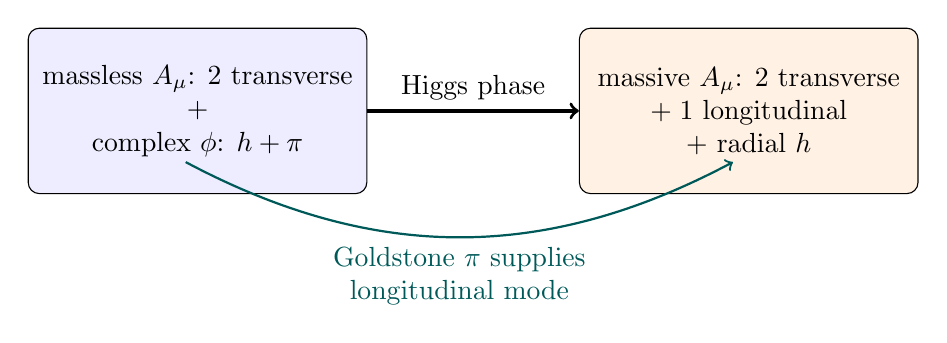
\begin{tikzpicture}[x=1cm,y=1cm]
  \node[draw,rounded corners,fill=blue!7,minimum width=4.3cm,
        minimum height=2.1cm,align=center] (before) at (0,0)
    {massless \(A_\mu\): \(2\) transverse\\
     \(+\)\\
     complex \(\phi\): \(h+\pi\)};
  \node[draw,rounded corners,fill=orange!10,minimum width=4.3cm,
        minimum height=2.1cm,align=center] (after) at (7,0)
    {massive \(A_\mu\): \(2\) transverse\\
     \(+\;1\) longitudinal\\
     \(+\) radial \(h\)};
  \draw[->,very thick] (before) -- node[above]{Higgs phase} (after);
  \draw[->,teal!70!black,thick]
    (-0.15,-0.65) to[bend right=28]
    node[below,align=center]{Goldstone \(\pi\) supplies\\longitudinal mode}
    (6.8,-0.65);
\end{tikzpicture}
\end{adjustbox}
\caption{Cơ chế Higgs sắp xếp lại, chứ không phá hủy, các bậc tự do
vật lý.}
\label{fig:l08-degree-rearrangement}
\end{figure}

\begin{classroomqa}
\audiencequestion{Làm sao bậc tự do góc có thể biến mất mà không
vi phạm phép đếm bậc tự do?\lecturetimestamp{01:19:13}}
\lecturerresponse{Nó không biến mất về mặt vật lý. Một vectơ không khối lượng có
hai helicity vì không thể đưa nó về trạng thái nghỉ. Một vectơ có khối lượng có
ba phân cực, gồm cả một phân cực dọc. Mode Goldstone trở thành
phân cực thứ ba đó, nên tổng số không đổi.}
\end{classroomqa}

Bài giảng đưa ra một phép kiểm tra động học hữu ích. Hãy hình dung một hạt vectơ có
khối lượng, làm chậm nó về trạng thái nghỉ, rồi tăng tốc nó theo một hướng mới.
Một phân cực từng là ngang đối với chuyển động ban đầu có thể trở thành dọc so với
chuyển động mới. Tương tự, nếu một hạt có khối lượng phân cực tròn được đưa qua
trạng thái nghỉ rồi cho chuyển động theo hướng ngược lại, nhãn helicity của nó sẽ
đảo ngược. Một hạt thực sự không khối lượng không thể được đưa qua thí nghiệm này,
vì không có hệ quy chiếu quán tính nào có thể đưa nó về trạng thái nghỉ. Do đó hai
helicity của nó tạo thành một phổ vật lý nhất quán.

\section{Phép tương tự trong siêu dẫn}

Trong một chất siêu dẫn thông thường, các electron tạo thành các cặp Cooper. Một cặp là một
boson mang điện tích \(2e\), và chất ngưng tụ được mô tả bởi một
tham số trật tự phức mang điện. Khi độ lớn của nó khác không,
tổ hợp giữa pha của nó và thế vectơ điện từ tạo ra
cơ chế Anderson--Higgs. Từ trường tĩnh suy giảm trên độ xuyên sâu London
thay vì kéo dài tự do xuyên qua phần khối. Theo nghĩa chính xác phụ thuộc môi trường này,
photon hành xử như thể nó đã thu được khối lượng.

Ví dụ này cũng làm sáng tỏ sự phân biệt ở phần mở đầu. Trường điện từ
không bị chuyển hóa vĩnh viễn thành một hạt cơ bản khác.
Quy luật lan truyền có khối lượng thuộc về trạng thái tập thể bên trong vật liệu;
ở bên ngoài, photon chân không vẫn không khối lượng.

\section{Những gì đã được xác lập}

Giờ đây có thể cô đọng lập luận mà không làm mất logic của nó:
\begin{enumerate}
  \item Một đối xứng liên tục toàn cục bị phá vỡ có một phương góc phẳng và
        do đó có một mode Goldstone không khối lượng.
  \item Tính bất biến pha cục bộ đòi hỏi một thế chuẩn và thay
        \(\partial_\mu\) bằng \(D_\mu\).
  \item Một hạng khối lượng trần \(A_\mu A^\mu\) vi phạm luật biến đổi cục bộ.
  \item Khi vô hướng mang điện có độ lớn cân bằng khác không \(f\), hạng
        bất biến chuẩn \(|D_\mu\phi|^2\) chứa
        \(\frac12g^2f^2A_\mu A^\mu\).
  \item Pha có thể bị loại bỏ bằng một lựa chọn chuẩn, và bậc tự do vật lý
        của nó trở thành phân cực dọc của vectơ có khối lượng.
  \item Kích thích Higgs hướng kính còn lại, với khối lượng được ấn định bởi độ cong
        của thế vô hướng.
\end{enumerate}

Nhiệm vụ tiếp theo là cho fermion khối lượng. Electron và quark không thể
trực tiếp dùng cơ chế vectơ; các ghép Higgs của chúng là những
tương tác Yukawa. Một khi vô hướng ổn định tại \(f\), các tương tác ấy trở thành
các hạng khối lượng fermion.

Phát biểu khái quát rằng các hạt quen thuộc sẽ không khối lượng nếu không có
sự phá vỡ đối xứng điện yếu cần thêm một điều lưu ý cuối cùng. Khối lượng
của các quark cơ bản và các lepton mang điện, cũng như khối lượng của \(W\) và \(Z\),
quả thật biến mất cùng với giá trị kỳ vọng Higgs. Tuy nhiên, phần lớn khối lượng của proton và neutron
phát sinh một cách động từ sự giam hãm QCD và năng lượng trường mạnh, chứ không phải từ khối lượng Higgs của các quark. Sự phân biệt đó không
làm thay đổi cơ chế Higgs được suy ra ở đây; nó giữ cho miền áp dụng của cơ chế ấy được chính xác.
